\begin{frame}[fragile]
  \frametitle{Control de flujo}

    \framesubtitle{Bucles}    

  \begin{itemize}
    \item Ciclo for...in
  \end{itemize}

  El ciclo for se utiliza como una forma gen\'erica de iterar sobre una secuencia.

  \begin{figure}
    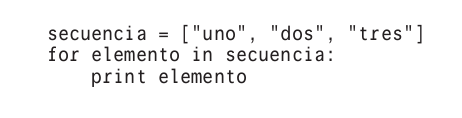
\includegraphics[width=0.6\textwidth]{Imagenes/For.jpg}
    \caption{\label{fig:Ejemplo8}Sintaxis de for...in en Python.}
  \end{figure}

\end{frame}
